\documentclass{article}
\usepackage{hyperref}
\usepackage{float}
\usepackage{tikz}
\usetikzlibrary{arrows.meta, positioning, calc, decorations.pathmorphing, shapes.geometric}
\begin{document}

\section{How To Use}
\begin{enumerate}
    \item Git clone seL4 from \href{https://github.com/SEL4/sel4}{seL4}.
    \item Setup sdfgen: \begin{enumerate}
        \item Clone microkit\_sdf\_gen from \href{https://github.com/au-ts/microkit_sdf_gen}{sdfgen}.
        \item Git checkout to the branch: joshua/unbacked\_mrs.
        \item Build the sdfgen library following the README.md instructions.
    \end{enumerate}
    \item Setup microkit: \begin{enumerate}
        \item Clone microkit from \href{git@github.com:au-ts/microkit.git}{microkit}.
        \item Git checkout to the branch joshua/send\_frames\_to\_pd.
        \item Build microkit following the DEVELOPER.md instructions.
        \item When building, use these flags: `--board=qemu\_virt\_aarch64 --configs=debug --skip-docs --skip-tar'
    \end{enumerate}
    \item Create LionsOS environment: \begin{enumerate}
        \item Clone \href{https://github.com/au-ts/lionsos}{LionsOS} 
        \item Git checkout to the branch joshua/userland\_pager.
        \item Copy the pager\_memory\_manager from examples.
        \item Add your applications, using the \texttt{mymalloc()} and \texttt{myfree()} functions and with a global variable int named \texttt{memory\_manager\_ep}.
        \item Create the \texttt{meta.py} file as one would normally.
        \item Inside the meta file, create a memory region with the backed argument as false for each application that uses \texttt{mymalloc()} and \texttt{myfree()}.
        \item Map these \textit{heaps} to each application.
        \item Create channels with ppc allowed from application to memory manager for each application that has a heap.
        \item Run the program. 
    \end{enumerate}
    
\end{enumerate}
\section{Implementation Details}

\begin{figure}[H]
    \centering
    
    
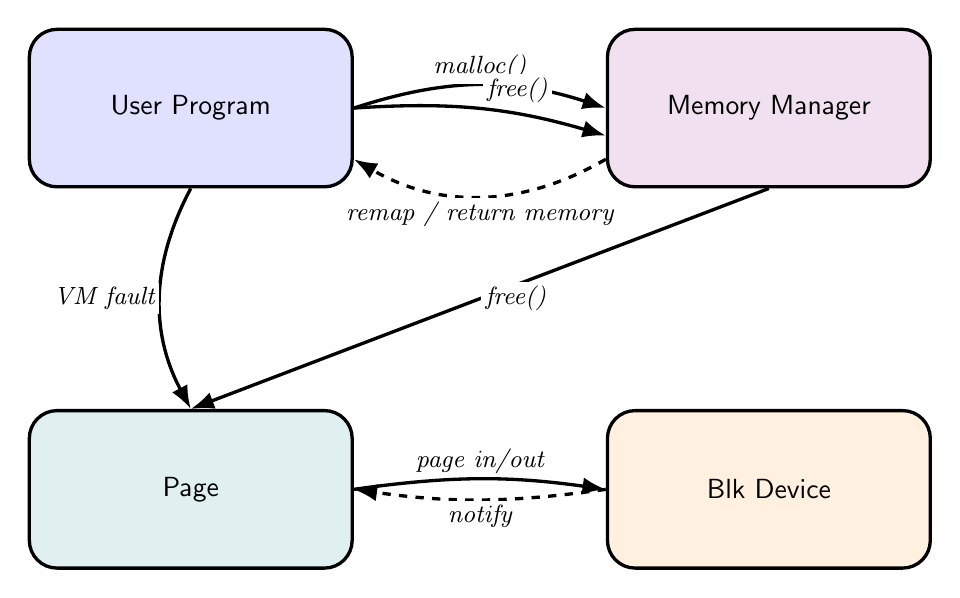
\begin{tikzpicture}[
font=\sffamily,
>=Latex,
node distance=2.8cm and 3.2cm,
box/.style={
draw,
rounded corners=10pt,
very thick,
minimum width=4.1cm,
minimum height=2.0cm,
align=center,
fill=#1!12
},
flow/.style={->, very thick},
backflow/.style={->, very thick, dashed},
lab/.style={midway, fill=white, inner sep=1.5pt, font=\small\itshape}
]

% Nodes
\node[box=blue] (user) {User Program};
\node[box=violet, right=of user] (mm) {Memory Manager};
\node[box=teal, below=of user] (page) {Page};
\node[box=orange, right=of page] (blk) {Blk Device};

% User <-> Memory manager
\draw[flow, bend left=18]
(user.east) to node[lab, above] {malloc()} (mm.west);

\draw[flow, bend left=10]
(user.east) to node[lab, above right] {free()} ($(mm.west)+(0,-0.35)$);

\draw[backflow, bend left=30]
($(mm.west)+(0,-0.65)$) to node[lab, below] {remap / return memory} ($(user.east)+(0,-0.65)$);

% User -> Page fault
\draw[flow, bend right=28]
(user.south) to node[lab, left] {VM fault} (page.north);

% Memory manager -> Page
\draw[flow]
(mm.south) -- node[lab, right] {free()} (page.north);

% Page <-> Block device
\draw[flow, bend left=8]
(page.east) to node[lab, above] {page in/out} (blk.west);

\draw[backflow, bend left=8]
(blk.west) to node[lab, below] {notify} (page.east);

\end{tikzpicture}

\caption{System Diagram for Pager and Memory Manager}
\end{figure}
\subsection{Design Problems}
LionsOS is a static operating system. What this means is that all applications and memory regions etc. are loaded before runtime and these applications run for the lifetime of the system. This forms a problem regarding the implementation of the pager and memory manager on LionsOS as the memory manager is supposed to grant extra memory to a protection domain on request. However, where should this memory come from? It is important to note that the microkit currently does not support the retyping of memory in userland. This means that it is impossible without extensively changing microkit to even change the page tables during runtime. The solution to this problem that I have come up with is to give each protection domain a memory region which acts like a heap. This heap is of course fixed in size, but through paging, we can have it such that the heap seems as large as required from the perspective of the protection domain. \textit{Note: this implementation is only a proof of concept design to run benchmarks to compare paging performance against Linux.}
\subsection{Limitations of the Design}
\begin{itemize}
    \item There is a static upper limit of the number of protection domains that are supported by the pager, defined as \texttt{MAX\_PDS}.
    \item Protection domains that are to be supported by the pager must be specified as `children' of the pager in the system description file.
    \item The `children' of the pager must have an ID less than \texttt{MAX\_PDS}.
    \item The memory manager only allocates 4k size blocks.
    \item The Pager must be named `pager' in the system description file.
    \item The number of available frames is fixed upon loading the system.
    \item The `heap' allocated to by the memory manager always starts at 0x8000000000.
    \item The `heap' must be specified in the system description file as an unbacked memory region. 
    \item Protection domains are singlethreaded.
    \item `Child' protection domains of the pager do not have other faults except page faults. 
\end{itemize} 
\subsection{Sdfgen}
In order to support such a heap described in section 2.1, we need to implement a memory region which actually remains unmapped from the vspace of the protection domain of the client. In order to do this, we need to have a flag in the memory region object of the system description file to mark a memory region to remain unmapped. This memory region also needs to have its frame caps to be accessible by and mapped into the pager protection domain to do paging operations. In order to support this, I have added a new optional boolean field identified as `backed'. By default memory regions are backed=true, and if they are backed=false, mappings are not done, only the page table structures are created, the memory region mapped to a protection domain named `pager' and the frame caps passed to the protection domain named `pager'. 
\\\\
This is implemented in \href{https://github.com/au-ts/microkit_sdf_gen}{sdfgen} in branch `joshua/unbacked\_mrs' as an additional optional field in the constructor of \texttt{MemoryRegion}. It is also possible to bypass the sdfgen entirely by writing up the system description file by hand and including an attribute `backed=false' in the memory region xml object.
\subsection{Microkit}
Microkit reads the SDF to load and run the system described in the SDF. I have modified microkit in order to implement the functionality described in the SDF.
\subsubsection{Special Protection Domains}
There are special protection domains which are named as below: \begin{itemize}
    \item pager
    \item memory\_manager
\end{itemize}
These are the required components to make the userland pager functional. The microkit when looping through the protection domains whilst building recognises these protection domain by their name string and implements special behaviour for these protection domains.
\paragraph{memory\_manager}
Any protection domains which has a ppc channel with memory manager should have a integer global variable named \textit{memory\_manager\_ep} as the microkit will on compile time write the ep number to this symbol. This will be used to do mymalloc and myfree function calls.
\paragraph{pager}
The pager needs to have all of the frames of the `heaps' mapped into its vspace and needs to have all of the frame caps in order to map the frames to the client protection domains' vspaces. Microkit usually loops through the memory regions, creates frame caps for them and maps the frames using these frame caps into their respective protection domains as specified by the mappings in the sdf. The modification which I have made in microkit intercepts the mapping of frames and checks whether or not the memory region is `backed', if not backed, the frame capability is stored in an array alongside with the id of the protection domain which the `heap' is mapped to. The frame is also mapped into the pager. The array is written as a symbol into the pager's elf so that the pager has access to the frame caps.
\subsubsection{Microkit Interface}
Wrapper functions were implemented for seL4\_ARM\_map/unmap functionality in microkit.h to allow the pager to do mapping operations.
\subsection{LionsOS}
LionsOS is used instead of microkit in order to have easier access to drivers through SDDF. 
\subsubsection{User Application}
The user application is very simple to implement. There should be a global integer variable \texttt{memory\_manager\_ep} which is passed to the functions \texttt{myfree()} and \texttt{mymalloc()} which can be found in \texttt{types.h}. These functions talk to the memory manager and \texttt{mymalloc()} returns the address of a 4k block of memory which is lazily mapped. \texttt{myfree()} frees the 4k memory block at the address provided as an argument.
\subsubsection{Memory Manager}
The memory manager implementation very simple for a proof of concept. Its role is to provide 4k blocks and to free these blocks. Given that malloc does not exist in LionsOS, we statically create an array of \texttt{struct mmap\_node}s which are given addresses starting from 0x8000000000, representing 4k blocks in memory. They can be indexed by their address rounded down to nearest 4k. There are also two doubly linked lists, one for used and unused blocked respectively. Each client protection domain has such an array and lists attributed to it.
\\\\
Upon intialisation, the nodes are all added to the unused list. When \texttt{mymalloc()} is called, a node is taken from the unused list and added to the used list. When \texttt{myfree()} is called, the node is found through indexing into the array of nodes using the address and that node is removed from the used list and added to the freed list. The memory manager also has a ppc ep with the pager and when free is called, a message is sent to the pager protection domain in order to wipe the pagefile slot and frame.
\subsubsection{Pager}
\paragraph{Data Structures}
There are two things the need to be kept track of: \textit{pagefile slots} \& \textit{frames/pages}.\\\\
The way that I keep track of pagefile slots is through an array. The slot index represents the position of the slot in the file. Essentially I abstract the pagefile as an array. There is a counter which represents the highest slot number which has ever been used so if a new file slot is required, that number can be given and incremented up. There is also a stack which track the freed slots from when a page is freed. If a slot is requested, the stack is checked first then the highest slot number is incremented.
\\\\
Instead of keeping track of page table entries as one normally would in a traditional pager implementation, since seL4 does not provide transparency into page tables, I have chosen to keep track of frame caps and a pseudo page table entry. pseudo page table entries are kept in an array of arrays, which are indexed by pd\_idx and address / 4096. The struct carrying the frame caps are what is used in the page replacement algorithm. They are stored in three lists, a free list, a inactive list and a active list.

\paragraph{Two List Page Replacement}
\begin{figure}[H]
    \centering
    \resizebox{1.3\textwidth}{!}{
        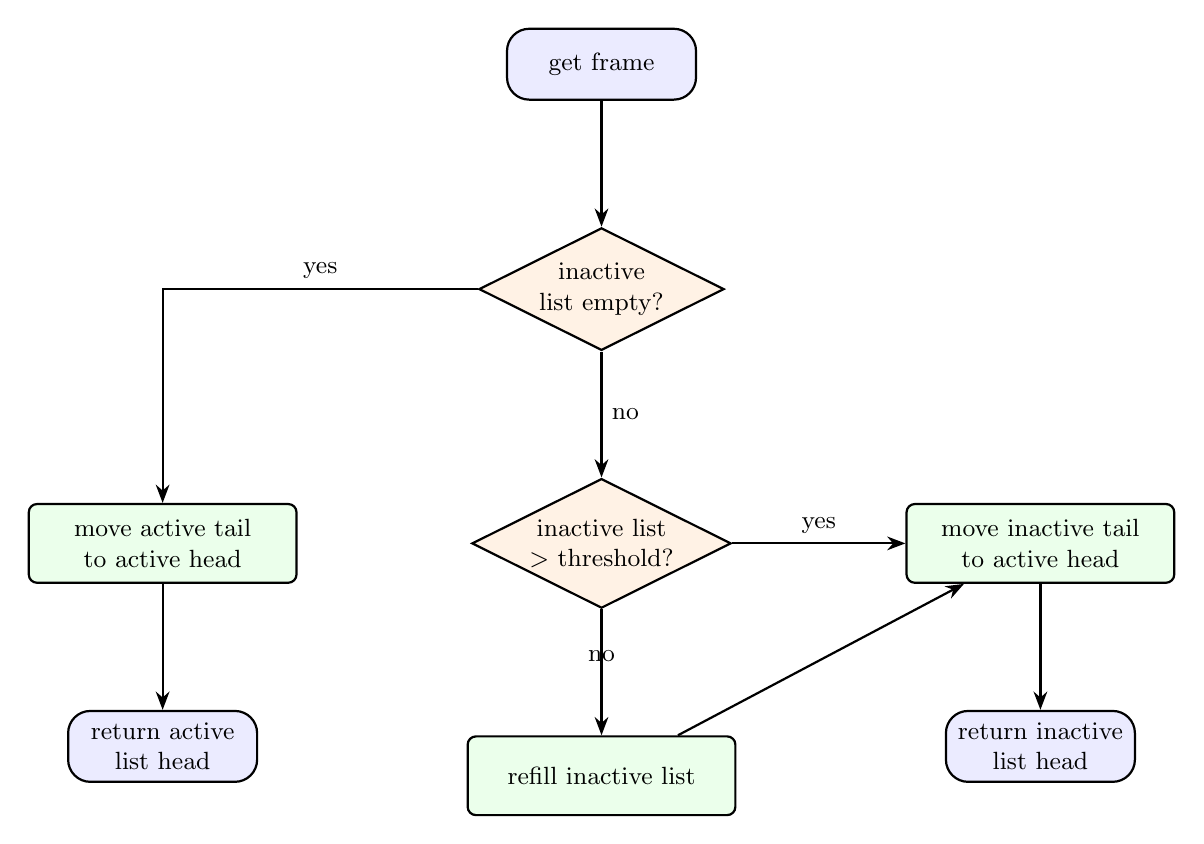
\begin{tikzpicture}[
node distance=16mm and 22mm,
font=\small,
>=Stealth,
startstop/.style={
rectangle, rounded corners=8pt,
draw, thick, align=center,
minimum width=24mm, minimum height=9mm,
fill=blue!8
},
process/.style={
rectangle,
draw, thick, rounded corners=3pt,
align=center,
minimum width=34mm, minimum height=10mm,
fill=green!8
},
decision/.style={
diamond,
draw, thick,
aspect=2,
align=center,
inner sep=1pt,
fill=orange!10
},
arrow/.style={->, thick}
]

\node[startstop] (start) {get frame};

\node[decision, below=of start] (inactiveEmpty)
{inactive\\list empty?};

\node[decision, below=of inactiveEmpty] (inactiveBig)
{inactive list\\$>$ threshold?};

\node[process, right=of inactiveBig] (moveInactive)
{move inactive tail\\to active head};

\node[startstop, below=of moveInactive] (returnInactive)
{return inactive\\list head};

\node[process, below=of inactiveBig] (refill)
{refill inactive list};

\node[process, left=of inactiveBig] (moveActive)
{move active tail\\to active head};

\node[startstop, below=of moveActive] (returnActive)
{return active\\list head};

\draw[arrow] (start) -- (inactiveEmpty);

\draw[arrow] (inactiveEmpty) -- node[right] {no} (inactiveBig);
\draw[arrow] (inactiveEmpty.west) -| node[pos=0.25, above] {yes} (moveActive.north);

\draw[arrow] (inactiveBig) -- node[above] {yes} (moveInactive);
\draw[arrow] (inactiveBig) -- node[above] {no} (refill);

\draw[arrow] (refill) -- (moveInactive);

\draw[arrow] (moveInactive) -- (returnInactive);

\draw[arrow] (moveActive) -- (returnActive);

\end{tikzpicture}


    }
    
\end{figure}
The entry point for the two list page replacement algorithm is the \texttt{get\_frame()} function which returns the next frame which could be used. This frame may or may not be already mapped to a page, but the pager takes care of that. The refill inactive function basically loops around the active list and if the current node's reference bit is set, sets this to false and unmaps and pushes to front of active list. If the current node is unreferenced then it is pushed to the front of the inactive list.
\paragraph{Paging Flow}
\begin{figure}[H]
    \centering
    \resizebox{1.3\textwidth}{!}{
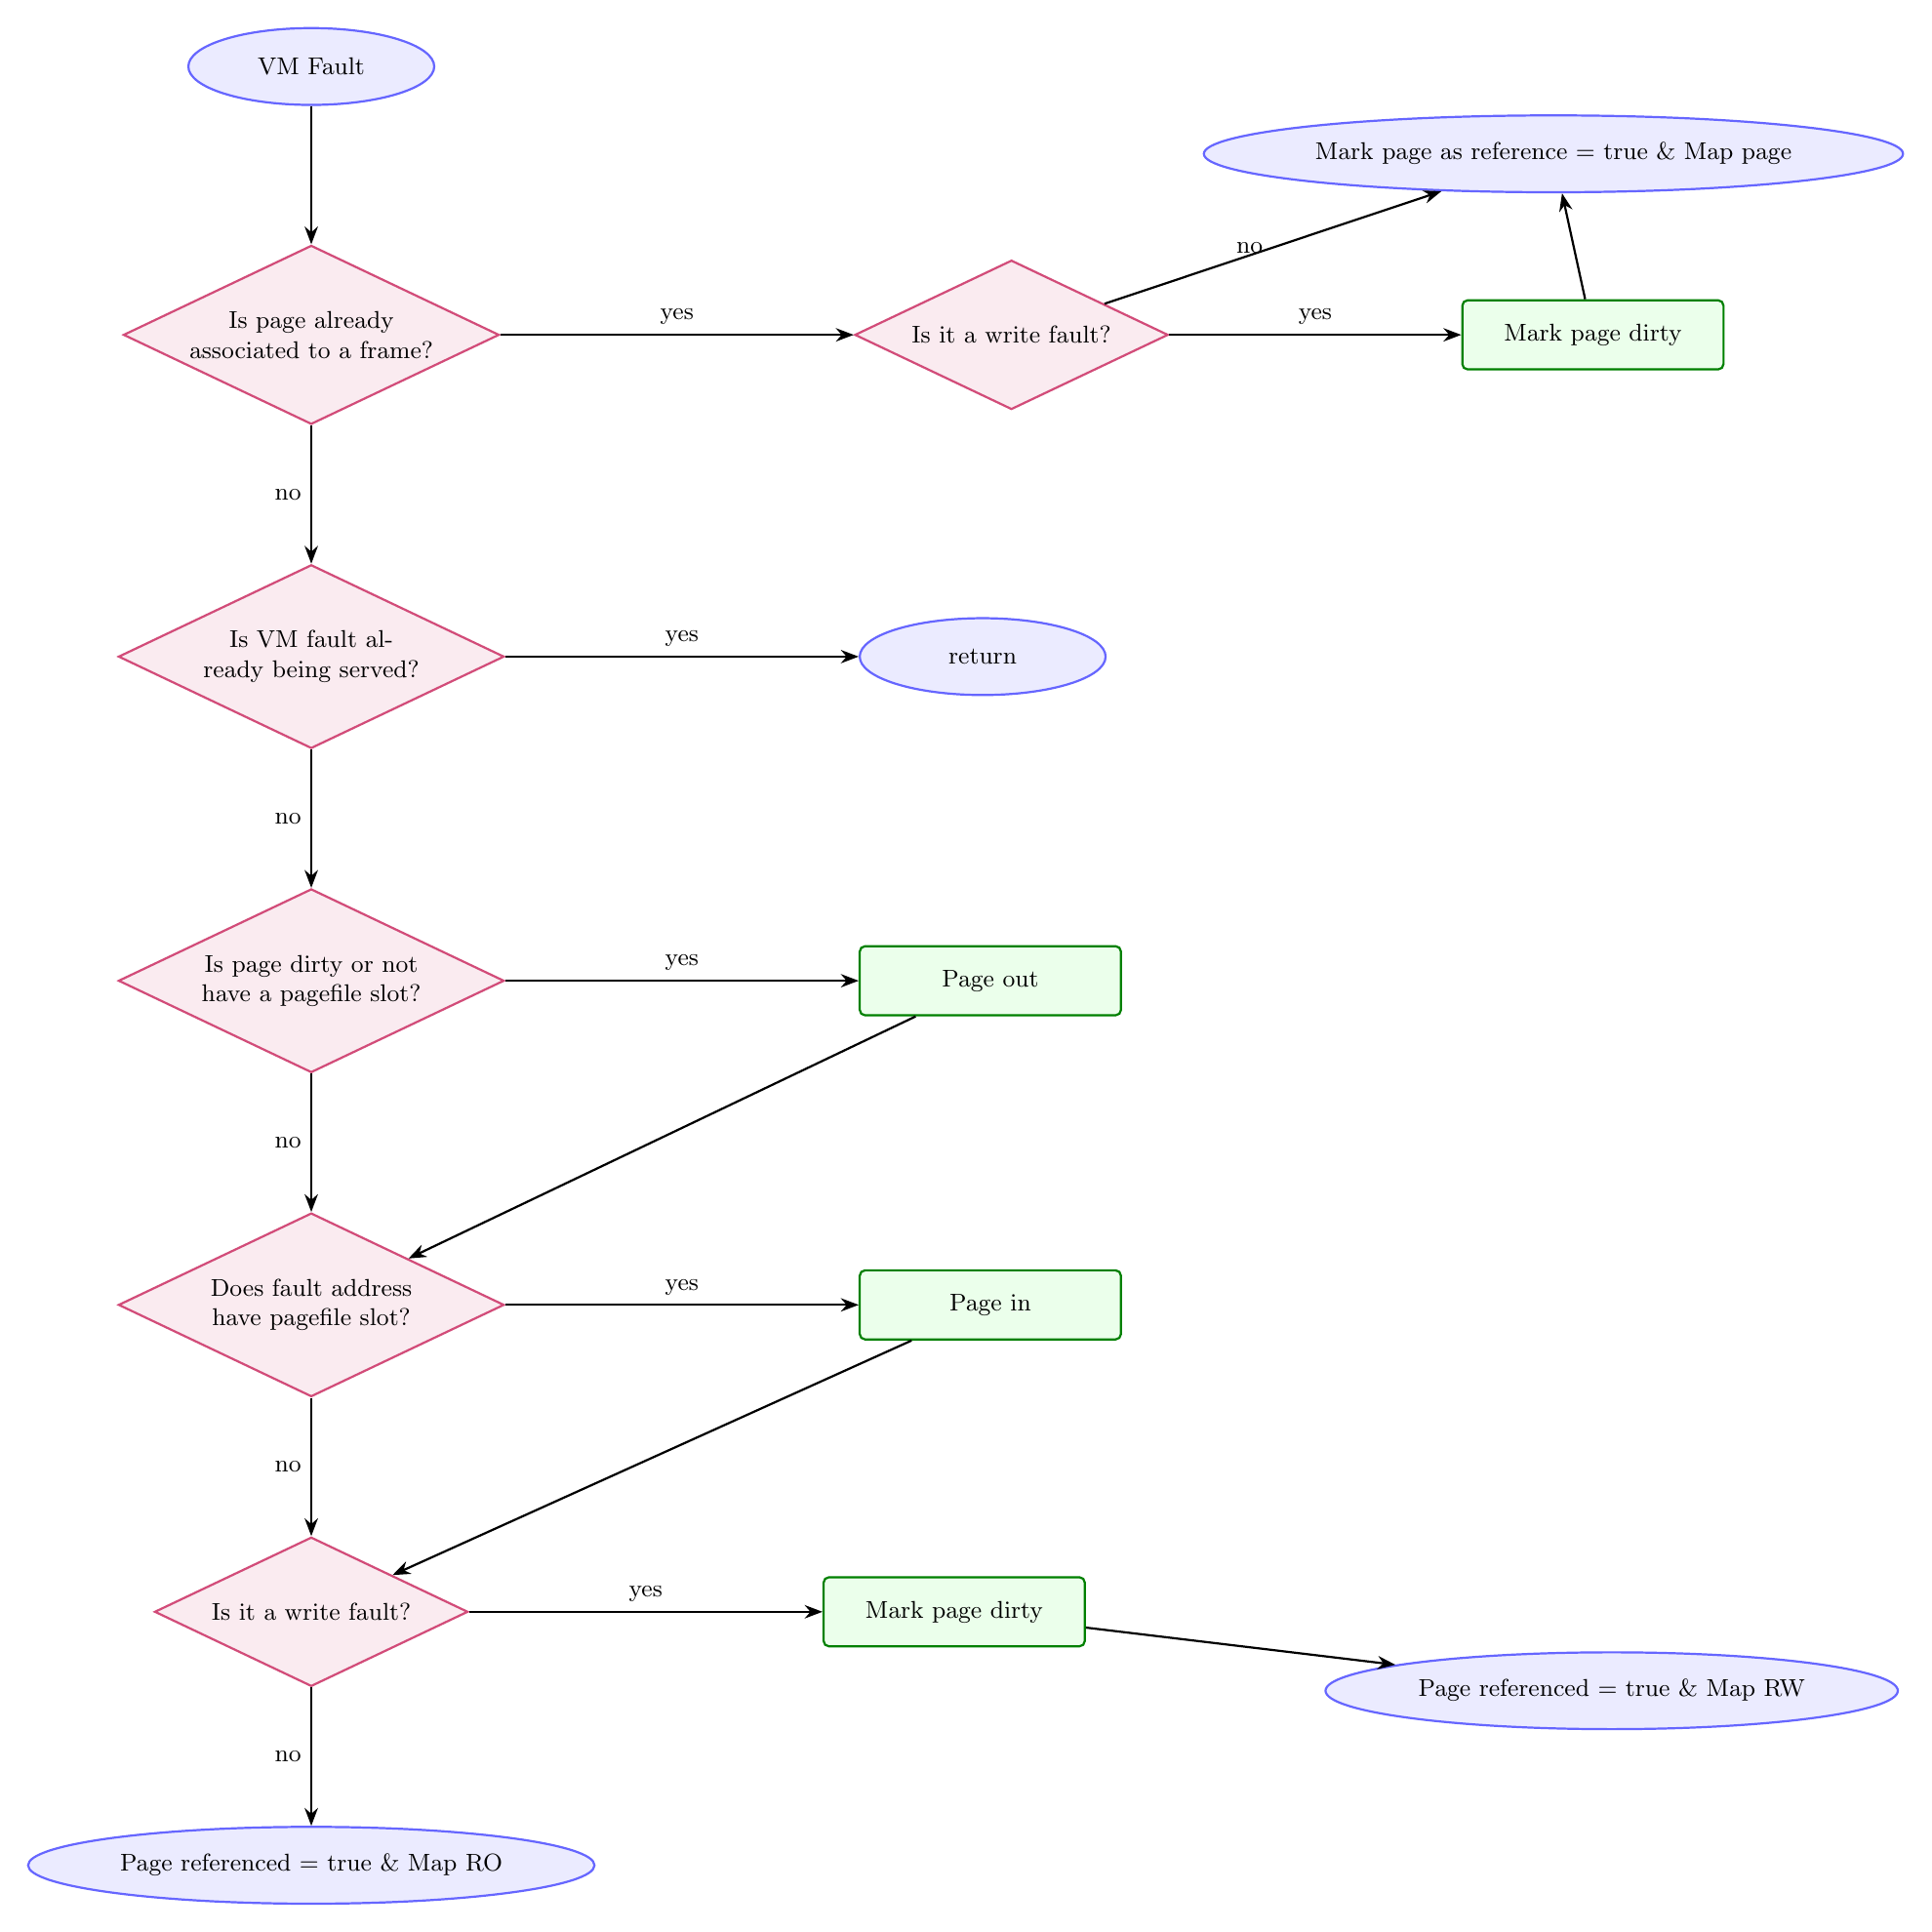
\begin{tikzpicture}[
node distance=1.8cm and 3.2cm,
>=Stealth,
every node/.style={font=\small},
startstop/.style={
ellipse,
draw=blue!60,
fill=blue!8,
thick,
minimum width=3.2cm,
minimum height=1cm
},
decision/.style={
diamond,
draw=purple!70,
fill=purple!8,
thick,
aspect=2.1,
inner sep=1pt,
text width=3.4cm,
align=center
},
process/.style={
rectangle,
rounded corners=2pt,
draw=green!50!black,
fill=green!8,
thick,
minimum width=3.4cm,
minimum height=0.9cm,
text centered
},
line/.style={draw, thick, ->}
]

% Nodes
\node[startstop] (fault) {VM Fault};

\node[decision, below=of fault] (assoc)
{Is page already associated to a frame?};

\node[decision, right=4.6cm of assoc] (writefault1)
{Is it a write fault?};

\node[startstop, above right=1.5cm and 2.8cm of writefault1] (mapframe)
{Mark page as reference = true \& Map page};

\node[process, right=3.8cm of writefault1] (dirty1)
{Mark page dirty};

\node[decision, below=of assoc] (handling)
{Is VM fault already being served?};

\node[startstop, right=4.6cm of handling] (return)
{return};

\node[decision, below=of handling] (pagedout)
{Is page dirty or not have a pagefile slot?};

\node[process, right=4.6cm of pagedout] (pageout)
{Page out};

\node[decision, below=of pagedout] (slot)
{Does fault address have pagefile slot?};

\node[process, right=4.6cm of slot] (pagein)
{Page in};

\node[decision, below=of slot] (writefault2)
{Is it a write fault?};

\node[process, right=4.6cm of writefault2] (dirty2)
{Mark page dirty};

\node[startstop, below right=0.2cm and 4.2cm of dirty2] (maprw)
{Page referenced = true \& Map RW};

\node[startstop, below=1.8cm of writefault2] (mapro)
{Page referenced = true \& Map RO};

% Connections
\draw[line] (fault) -- (assoc);

% already associated branch
\draw[line] (assoc) -- node[above] {yes} (writefault1);

\draw[line] (writefault1) -- node[above] {yes} (dirty1);
\draw[line] (dirty1) -- (mapframe);

\draw[line] (writefault1) -- node[left] {no} (mapframe);

% not associated branch
\draw[line] (assoc) -- node[left] {no} (handling);

\draw[line] (handling) -- node[above] {yes} (return);
\draw[line] (handling) -- node[left] {no} (pagedout);

\draw[line] (pagedout) -- node[above] {yes} (pageout);
\draw[line] (pageout) -- (slot);

\draw[line] (pagedout) -- node[left] {no} (slot);

\draw[line] (slot) -- node[above] {yes} (pagein);
\draw[line] (pagein) -- (writefault2);

\draw[line] (slot) -- node[left] {no} (writefault2);

\draw[line] (writefault2) -- node[above] {yes} (dirty2);
\draw[line] (dirty2) -- (maprw);

\draw[line] (writefault2) -- node[left] {no} (mapro);

\end{tikzpicture}}
\end{figure}
Paging follows the flow shown above, except that paging in and out operations are done asynchronously through the blk driver. We facilitate this by having a \texttt{page\_continuations} array which allows the pager to index into using the child id and store the paging data which contains the frame, child id, fault address and a enum which tells the pager when notified that the blk operation is finished whether it was a page in or out. There is also a similar array of integers named \texttt{current\_faults} also indexed by child id that stores the fault address to make sure that the current fault is not serviced multiple times. Since we assume that PD's are singlethreaded, there should only be one VM fault happening at any time for a single PD. 
\end{document}